
% poster settings
\documentclass[17pt, a1paper, portrait, margin=0mm, innermargin=15mm,
     blockverticalspace=15mm, colspace=15mm, subcolspace=8mm]{tikzposter}

% \tikzposterlatexaffectionproofon %shows small comment on how the poster was made at bottom of poster

%% changing the fonts
\usepackage{cmbright}
%\usepackage[default]{cantarell}
%\usepackage{avant}
%\usepackage[math]{iwona}
\usepackage[math]{kurier}
\usepackage[T1]{fontenc}
\usepackage{array}
\usepackage{tabularx}
\usepackage{graphicx,float}

\tikzposterlatexaffectionproofoff
%% add your packages here


\usepackage{hyperref}
\usepackage{mathtools}
\usepackage{listings,xcolor}
\usepackage{amsfonts}

% title format

\settitle{ 
  	%Title
  	\begin{minipage}{0.2\linewidth}
		\phantom{xxxxxxxxxxxxxxxxxxxxxxxxxxxxxxxxxxx}
  	\end{minipage}
	\begin{minipage}[c]{0.4\linewidth}
		 %\begin{center} 
		 \vbox{
			\color{titlefgcolor} {\bfseries \Huge \sc \@title \par}
     		\vspace*{1em}
     		{\huge \@author \par} 
			\vspace*{1em} 
			{\LARGE \@institute}
		}
		%\end{center}
  	\end{minipage}
	% Right logo
	\begin{minipage}[c]{0.37\linewidth}
		\centering 
 			\@titlegraphic
  	\end{minipage}
}



 % Commands
 
\newcommand{\kc}[1]{\texttt{\small #1}}
\let\cc\lstinline

 
\newcommand{\bs}{\textbackslash}   % backslash
\newcommand{\cmd}[1]{{\bf \color{red}#1}}   % highlights command

 % Title, Author, Institute
\title{An Executable Formal Semantics for PHP}
\author{Daniele Filaretti \& Sergio Maffeis} 
\institute{Department of Computing, Imperial College London}
\titlegraphic{
	\begin{tabular}{c>{\hspace{4pc}}c}
			$\vcenter{\hbox{
\includegraphics[scale=0.45]{img/imperial_trans.png}}}$
	\end{tabular}
}


\definecolorstyle{sampleColorStyle}{
     \definecolor{colorOne}{named}{blue}
     \definecolor{colorTwo}{named}{yellow}
     \definecolor{colorThree}{named}{orange}
 }{
     % Background Colors
     \colorlet{backgroundcolor}{colorOne!50!white}
     \colorlet{framecolor}{black}
     % Title Colors
     \colorlet{titlefgcolor}{black}
     \colorlet{titlebgcolor}{colorOne}
     % Block Colors
     \colorlet{blocktitlebgcolor}{colorTwo}
     \colorlet{blocktitlefgcolor}{black}
     \colorlet{blockbodybgcolor}{white}
     \colorlet{blockbodyfgcolor}{black}
     % Innerblock Colors
     \colorlet{innerblocktitlebgcolor}{colorOne!60!white}
     \colorlet{innerblocktitlefgcolor}{black}
     \colorlet{innerblockbodybgcolor}{white}
     \colorlet{innerblockbodyfgcolor}{black}
     % Note colors
     \colorlet{notefgcolor}{black}
     \colorlet{notebgcolor}{colorThree!50!white}
     \colorlet{noteframecolor}{colorTwo}
     % ColoredBox   
     \colorlet{coloredboxfgcolor}{blue}
     \colorlet{coloredboxbgcolor}{colorThree!10!white}
     \colorlet{coloredboxframecolor}{colorOne}
}
 
%Theme: {Default, Basic, Rays, Simple, Envelope, Wave, Board, Autumn, Desert}
\usetheme{Board}
\usecolorstyle[colorPalette=Default]{sampleColorStyle}


\begin{document}
	\maketitle
	
	% Row 1 : Intro
	\begin{columns}
		\column{1}
			\block{Motivation} {
					
			\begin{tabular}[t]{ccc}
      			
      		
		\begin{minipage}[c]{.5\linewidth}	
				\textbf{PHP is among the most popular programming languages}
				and it is the 
				most common choice for server-side scripting.
				It powers applications such as Facebook, Yahoo, 
				Wikipedia and Wordpress and, not surprisingly,
				it is the place where most vulnerabilities in web application are
				found.
				Vulnerabilities such as XSS and SQLi
				are an ideal target for static analysis, but
				PHP is notoriously \textbf{hard to analyse} 
				(due to its dynamic features).
				Its semantics is poorly understood 
				by both developers and security specialists, and
				the \textbf{absence of a written language specification}
				or  even of a
				detailed and comprehensive documentation doesn't help.  
				As a result, \textbf{existing bug-finding tools 
				don't provide any formal guarantee of soundness or coverage}
				and miss many existing bugs.	
				Our goal is to develop a new generation of
				semantics-based static analysis tools targeting 
				web application security, based on a rigorous  
				formal model of the PHP language. 
      		\end{minipage}
			
			&
			
			\begin{minipage}[c]{0.5\linewidth}			
			
			\begin{center}
				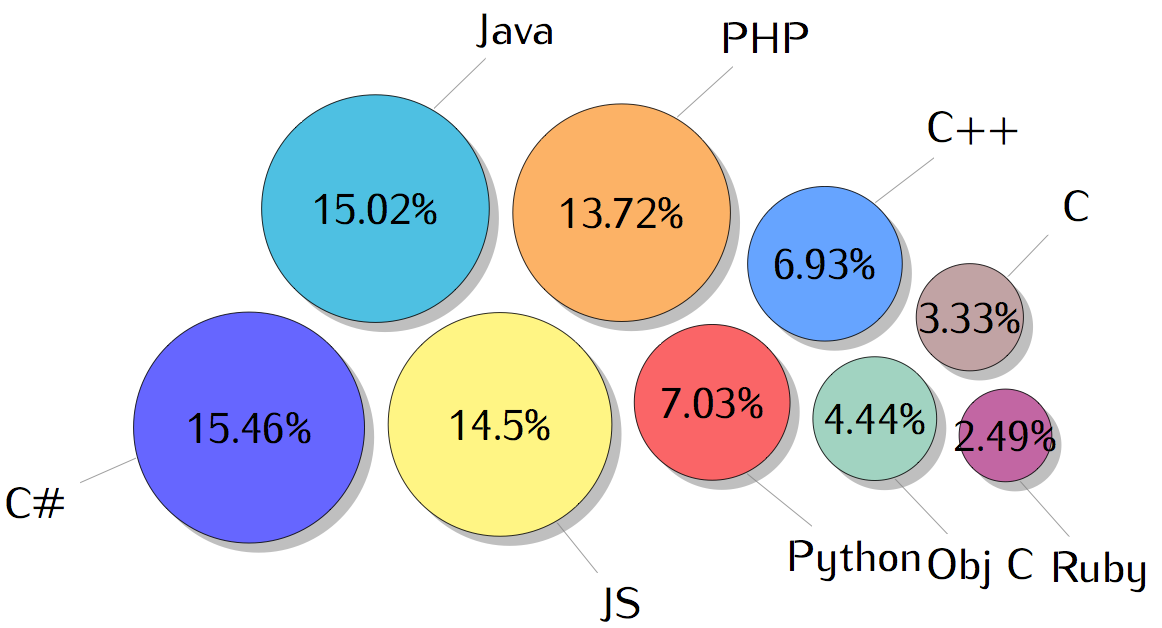
\includegraphics[scale=0.5]{img/lang-pop.png}
			\end{center}
		
			

			\end{minipage}
			
		\end{tabular}
		\vspace{17pt}
		\begin{center}

			\begin{tabular}{c>{\hspace{5pc}}c>{\hspace{5pc}}c>{\hspace{5pc}}c}
				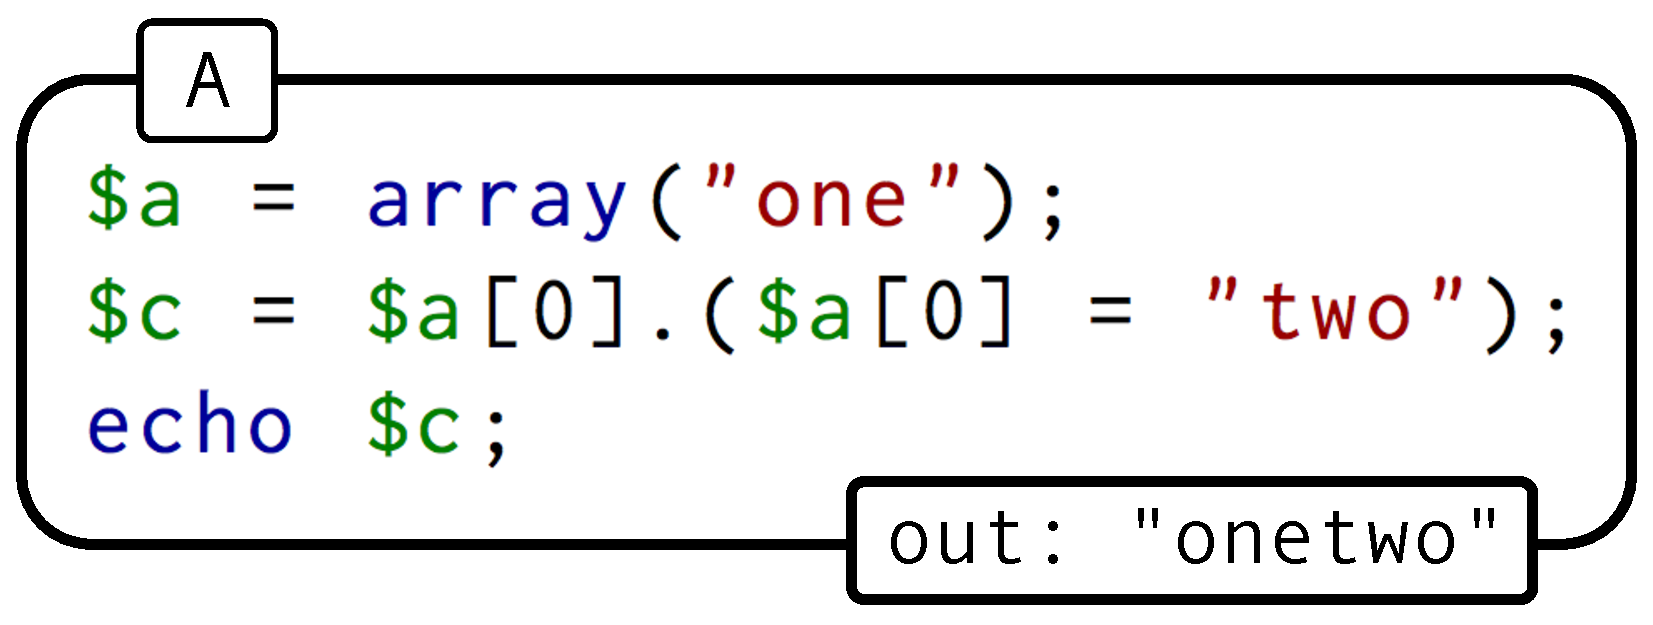
\includegraphics[scale=0.4]{img/code-ex-1.pdf}     
				& 
				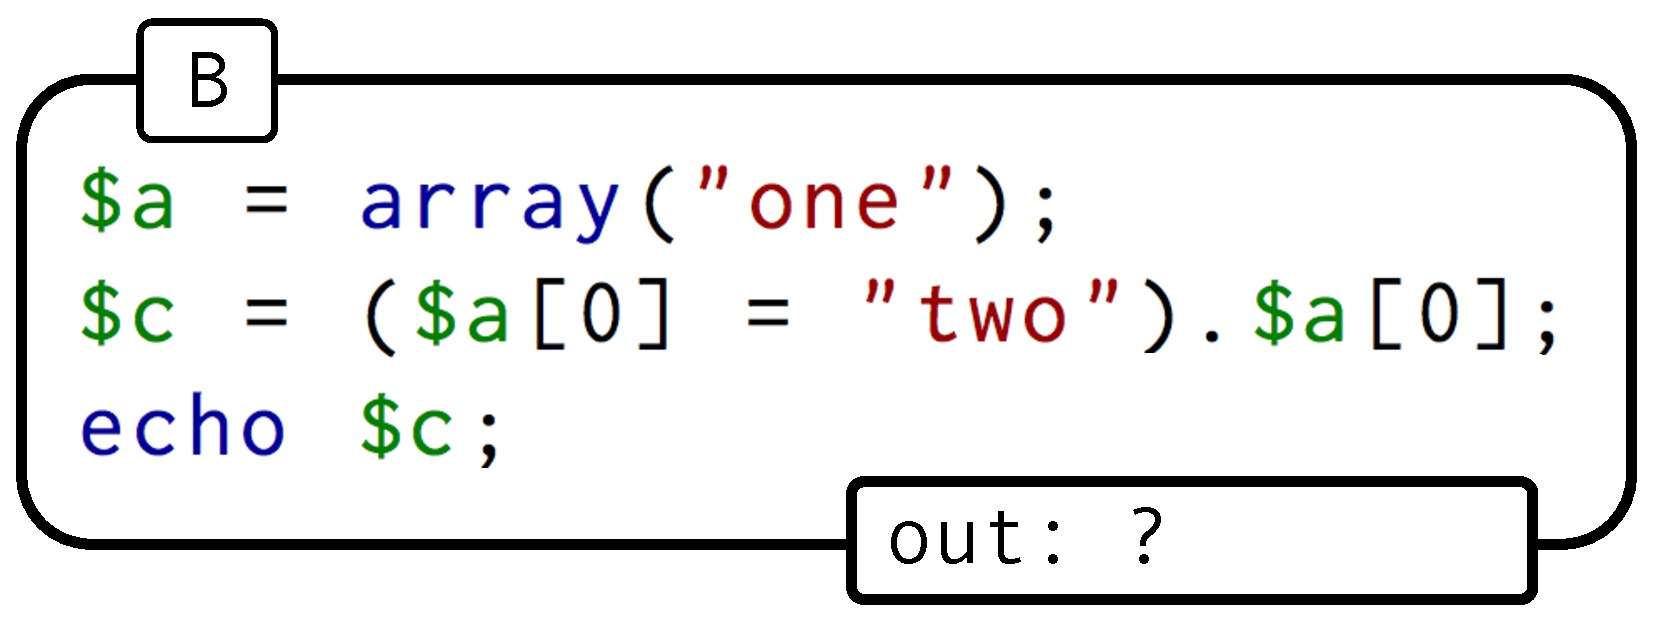
\includegraphics[scale=0.4]{img/code-ex-2.pdf}
				& 
				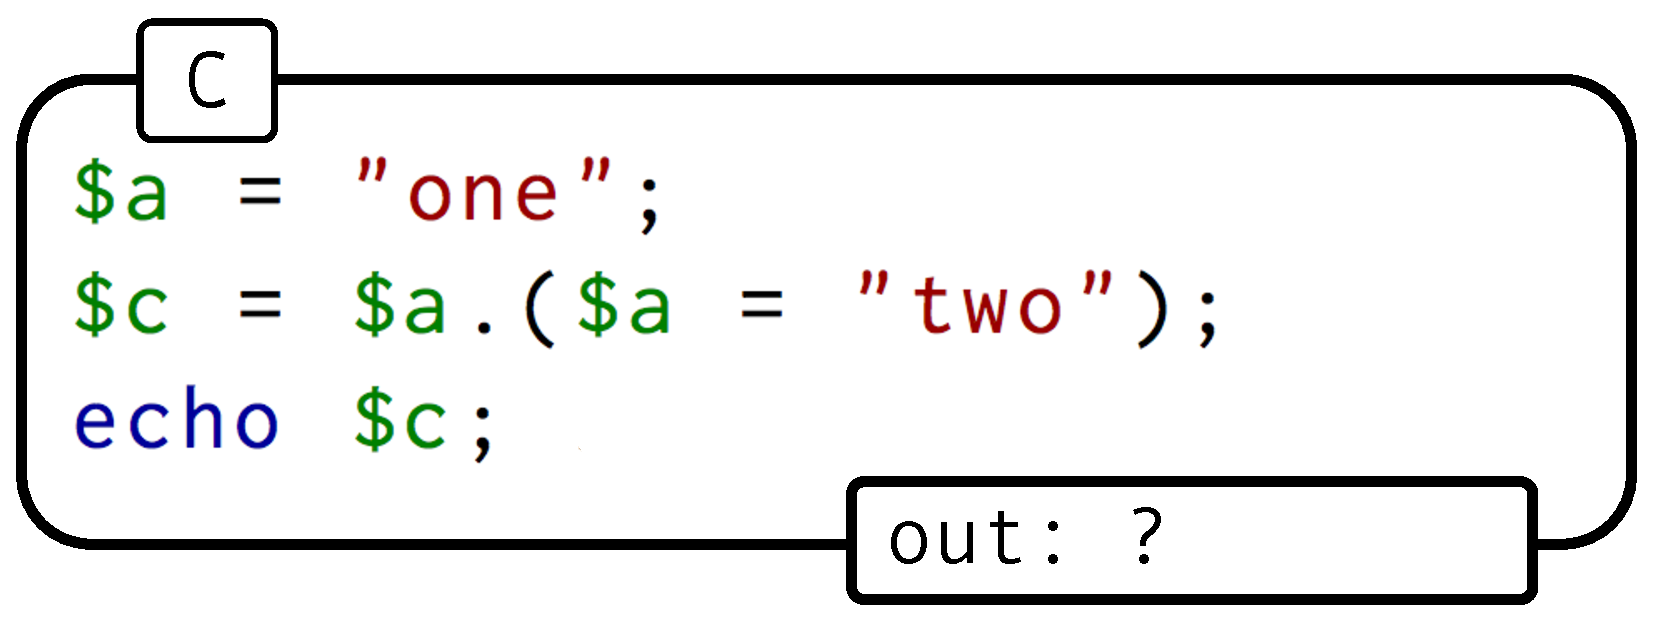
\includegraphics[scale=0.4]{img/code-ex-3.pdf}
				& 
				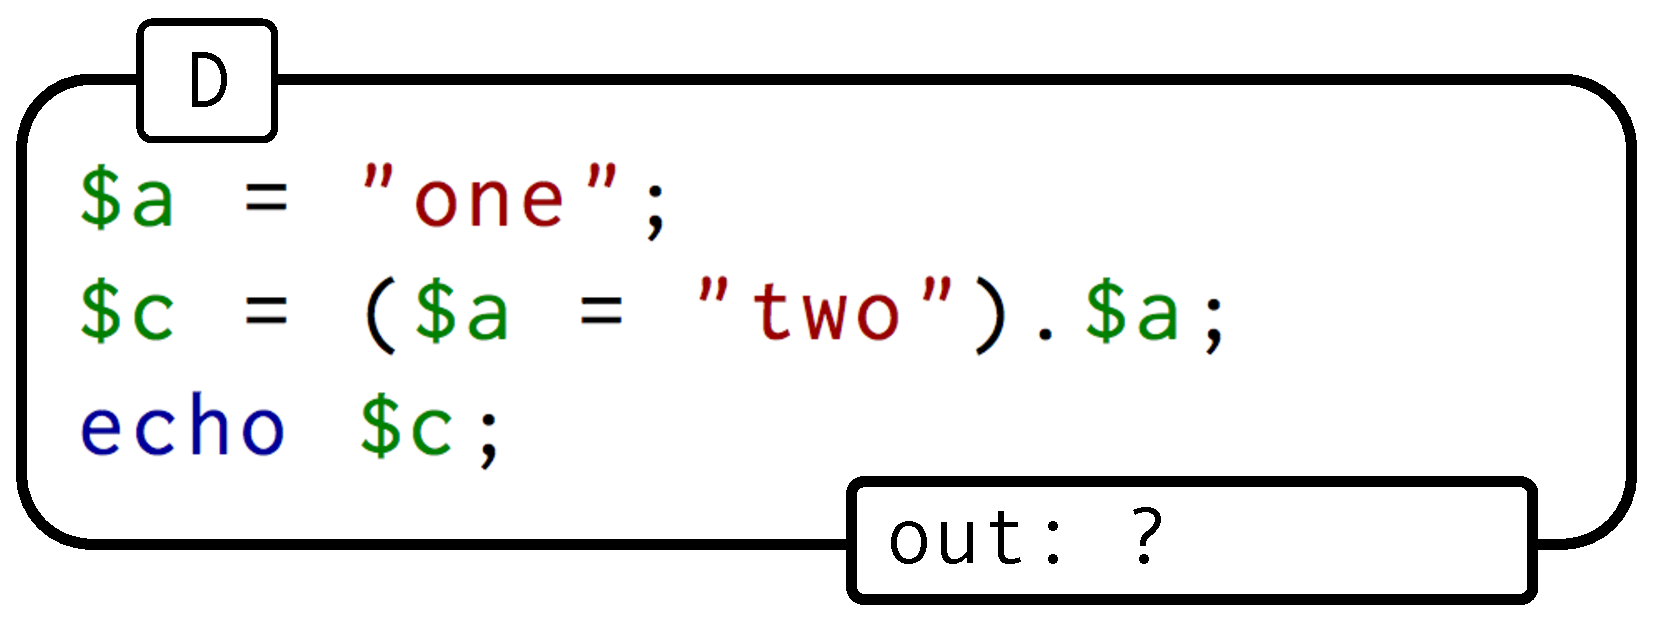
\includegraphics[scale=0.4]{img/code-ex-4.pdf}	
				\end{tabular}
			\end{center}	
	}		
			
	\end{columns}
	
	% Row 2: our approach - method
	\begin{columns}
		
		\column{1}
			\block{$\mathbb{K}$PHP: formalising PHP in $\mathbb{K}$}{
				
				\begin{tabular}[t]{ccc}
					\begin{minipage}[c]{0.5\linewidth}
						\coloredbox[bgcolor=white, framecolor=white]{
						We formalise PHP in $\mathbb{K}$, a semantics 
						framework based on rewriting logic and 
						implemented on top of the Maude system. 
						States, or \emph{configurations}, are represented as
						labeled, possibly nested \emph{cells}, each 
						containing part of the program state  
						(e.g.: fragments of program, stacks, environments, function 
						definitions etc.).
						\vspace{17pt}
						\begin{center}
							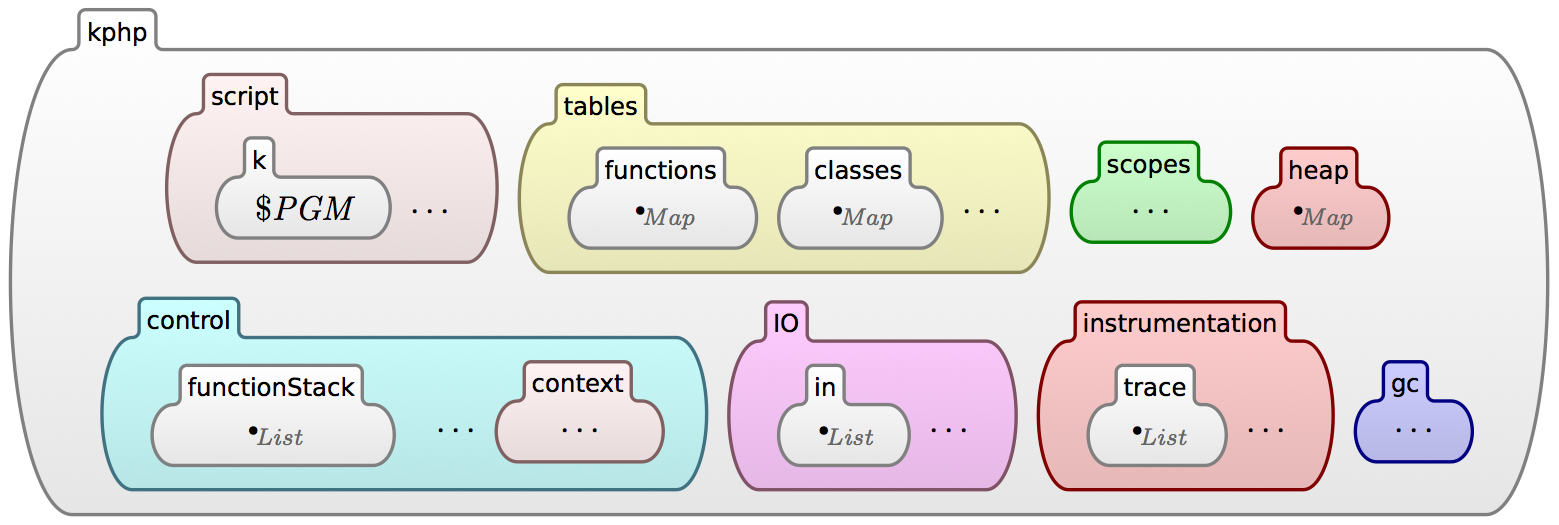
\includegraphics[scale=0.48]{img/config.png}
      					\end{center}
						After a program is placed into the \texttt{k} cell,
						the rewrite rules can be applied,  
						causing transitions to new configurations.
						A $\mathbb{K}$ semantics has a rigorous meaning 
						as a term rewriting system, hence it is suitable for 
						formal reasoning.
						It is also \textbf{directly executable}, enabling a 
						tight design/test loop.
						The $\mathbb{K}$/Maude tool-chain provides support for
						\textbf{LTL model checking and symbolic execution}.
					}
				\end{minipage}
					&  
					\begin{minipage}[c]{0.5\linewidth}
					
					\innerblock[
						titleoffsety=0pt, 
						bodyoffsety=0pt, 
						bodywidthscale=.95, 
						titlewidthscale=.95]{$\mathbb{K}$ rules}{
					$\mathbb{K}$ rules can be \emph{computational} or 
					\emph{structural}. Computational rules give meaning to 
					atomic constructs. They apply once all subterms are in the 
					desired form and cause a state transition.
					\vspace{17pt}
						\begin{center}
							\begin{tabular}{rlll}
								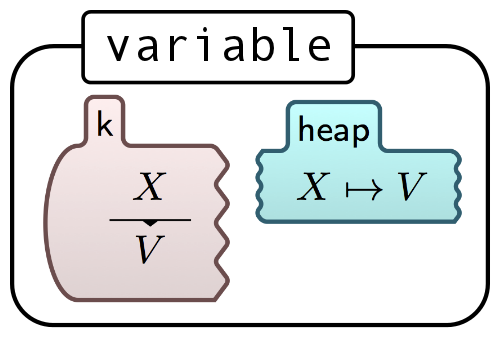
\includegraphics[scale=0.42]
									{img/rule-framed-variable.png}   
								& 
								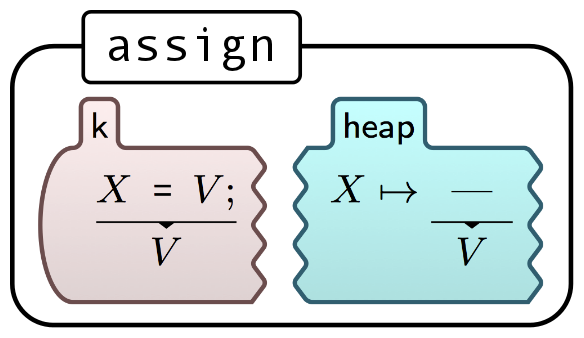
\includegraphics[scale=0.42]
									{img/rule-framed-schema.png}
								& \\
								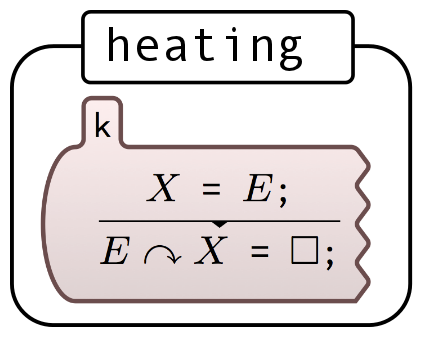
\includegraphics[scale=0.42]
									{img/rule-framed-heating.png}  
								&
								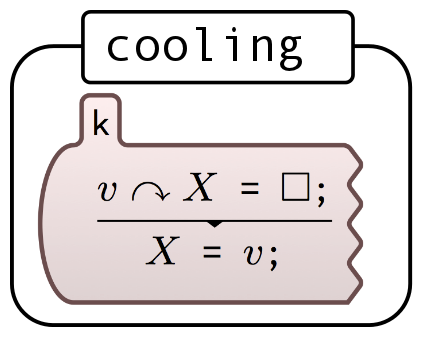
\includegraphics[scale=0.42]
									{img/rule-framed-cooling.png}
							\end{tabular}
						\end{center}							
					\emph{Heating} and \emph{cooling} rules are examples of 
					\emph{structural} rules. Their role is to define 
					evaluation strategies and they don't count as 
					computational steps.
					}
      				\end{minipage}
				\end{tabular}
				
						
			\begin{center}
					\begin{tabular}{ccccccccc}
						$\vcenter{\hbox{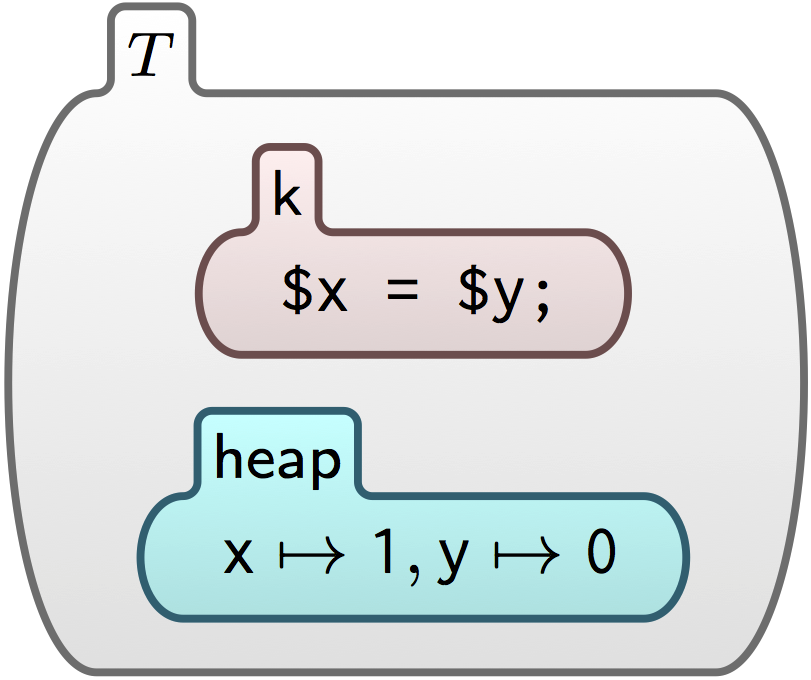
\includegraphics[scale=0.25]
						{img/state-1.png}}}$
						& 
						\begin{tabular}{c}
						{\color{red}heating} \\
						$\Longrightarrow$
						\end{tabular}
						&
						$\vcenter{\hbox{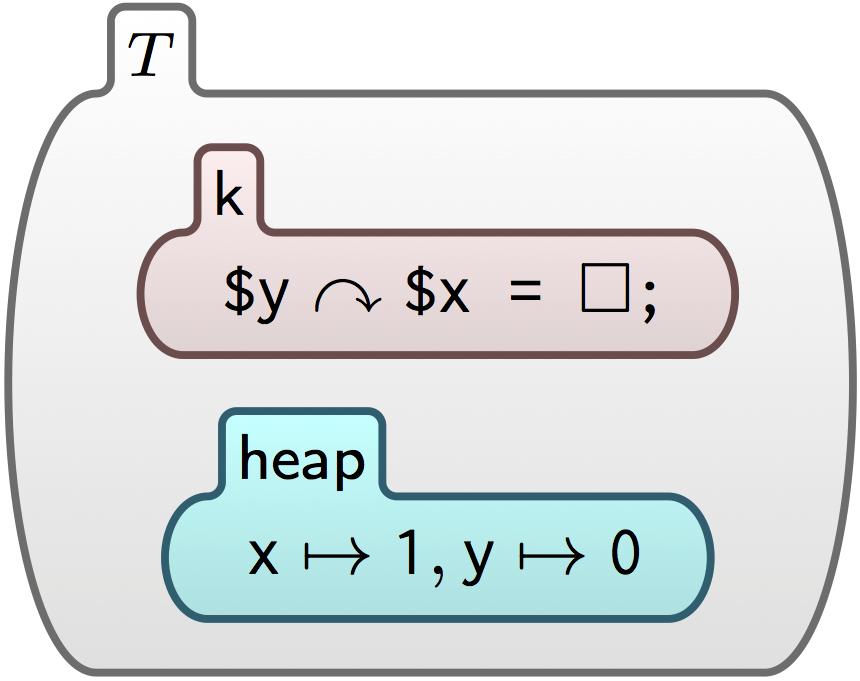
\includegraphics[scale=0.25]
						{img/state-2.png}}}$
						&
						\begin{tabular}{c}
							variable \\
							$\Longrightarrow$
						\end{tabular}
						& 
						$\vcenter{\hbox{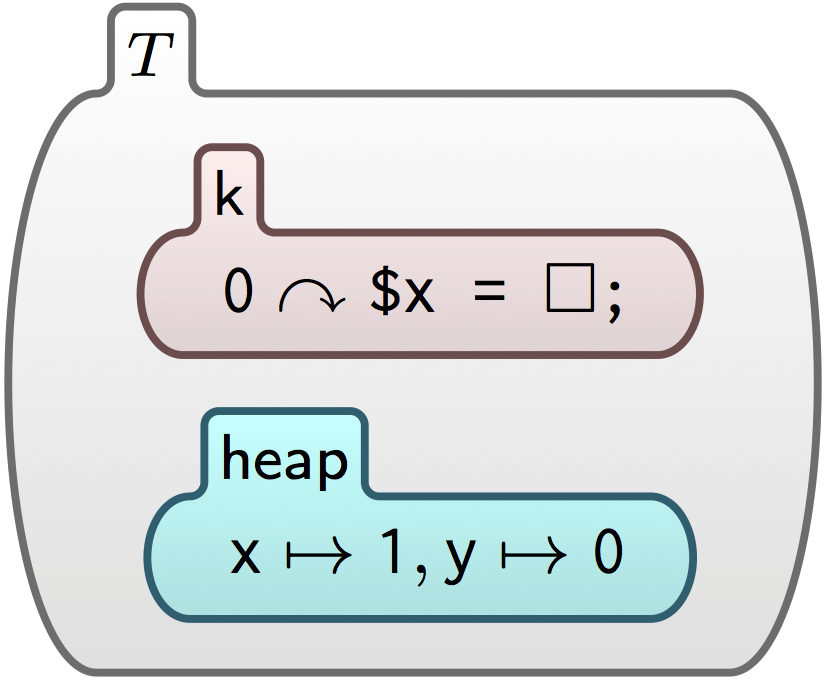
\includegraphics[scale=0.25]
						{img/state-3.png}}}$
						&
						\begin{tabular}{c}
							{\color{blue}cooling} \\
							$\Longrightarrow$
						\end{tabular}
						& 
						$\vcenter{\hbox{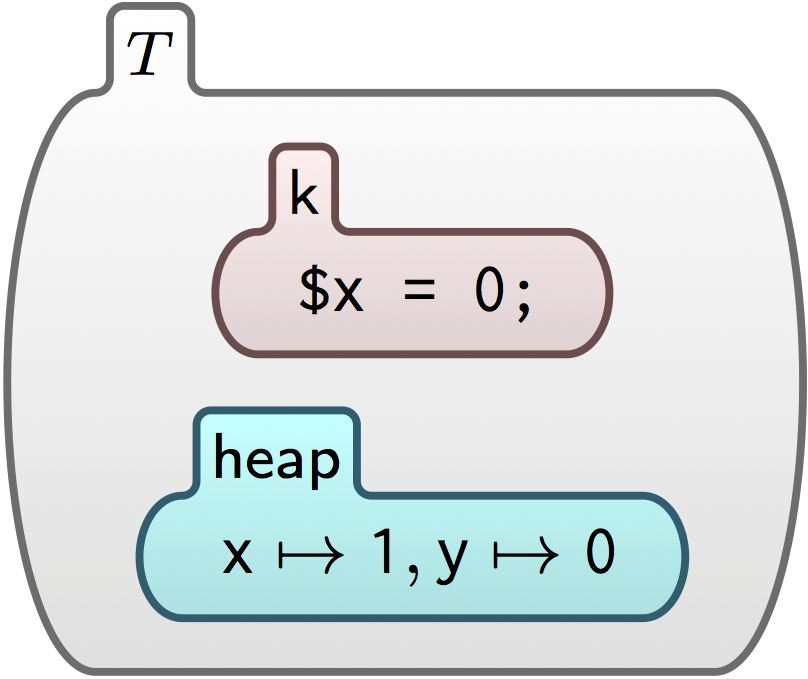
\includegraphics[scale=0.25]
						{img/state-4.png}}}$
						&
						\begin{tabular}{c}
							assign \\
							$\Longrightarrow$
						\end{tabular}
						&
						$\vcenter{\hbox{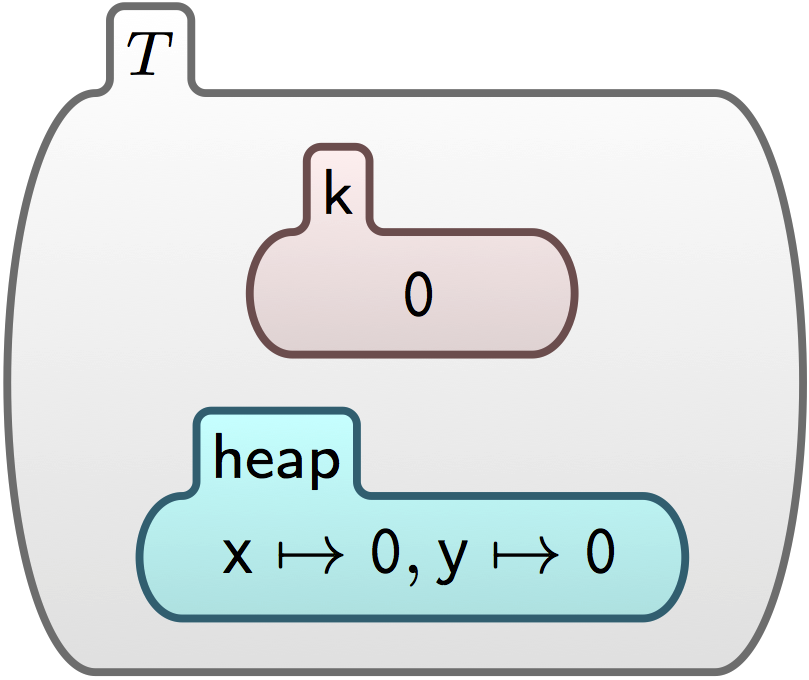
\includegraphics[scale=0.25]
						{img/state-5.png}}}$
					\end{tabular}
					\end{center}
%		}\note[targetoffsetx=500pt, targetoffsety=0pt]{
%			
		}



		
			
	\end{columns}
	
	
	% Row 3: results - applications
	
	\begin{columns}
		\column{0.5}
			\block{$\mathbb{K}$PHP Interpreter and validation}{
				\begin{tabular}[t]{cc}
					\begin{minipage}[c]{0.5\linewidth}
						The executable semantics doubles as a PHP interpreter. 
						We validate 
						our formalisation by \textbf{passing all the tests 
						for the official PHP Zend implementation} targeting  
						the portion of the language we cover.
						To improve coverage, we augment the test 
						suite with additional  cases.
						$\mathbb{K}$PHP, together with a web interface and examples
						are available online at \texttt{http://phpsemantics.org}.
					\end{minipage}
					& 
					\begin{minipage}[c]{0.5\linewidth}
						\begin{center}
							
							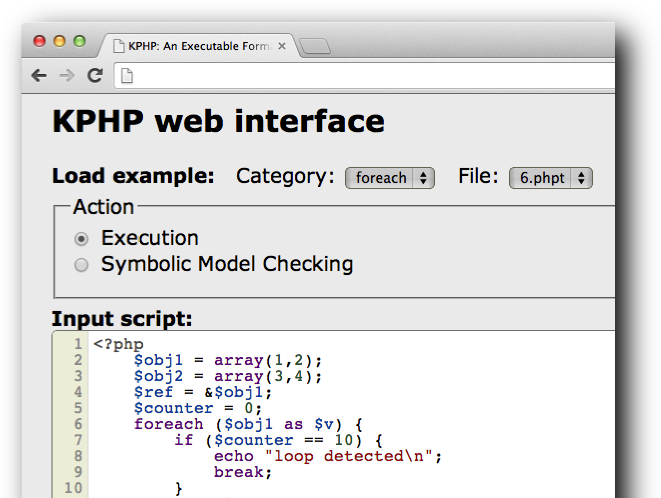
\includegraphics[scale=.5]{img/screenshot-shadow-cut.png}
						\end{center}
					\end{minipage}
				\end{tabular}
			}
			\block{References}{
				\textbullet \phantom{.}
				D.Filaretti \& S.Maffeis, \emph{An Executable Formal Semantics
				for PHP}, ECOOP'14. \\
				\textbullet \phantom{.}
				G. Rosu, \emph{$\mathbb{K}$ Overview and SIMPLE Case Study}, ENTCS'13
				%\centering Work funded by EPSRC grant EP/I004246/1
			}
			\note[targetoffsetx=750px, targetoffsety=-10px, width=400pt]{Work funded by EPSRC grant EP/I004246/1}
			
			
		\column{0.5}
			\block{Analysis of PHP programs} {
				\begin{tabular}[t]{cc}
					\begin{minipage}[c]{0.5\linewidth}
						\innerblock[
							titleoffsety=0pt, 
							bodyoffsety=0pt, 
							bodywidthscale=.95, 
							titlewidthscale=.95]{LTL model checking}{
							By \textbf{extending LTL} with predicates 
							over configurations we are able to verify 
							properties of PHP program.
							\vspace{17pt}
							\begin{center}
								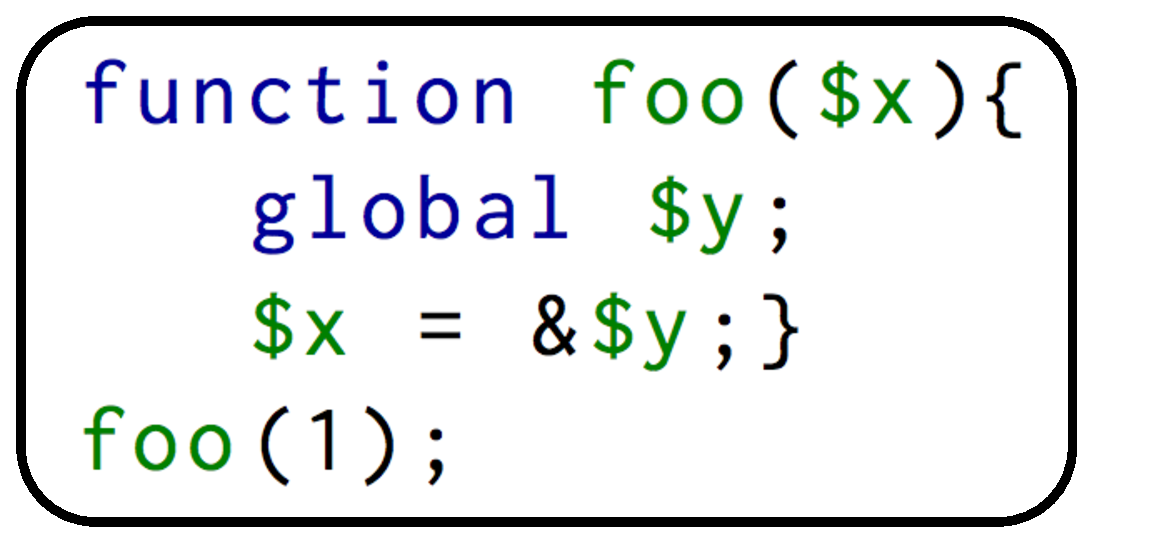
\includegraphics[scale=0.4]{img/code-ltl.pdf}
							\end{center} 
							{\color{white}a}		% FIX THIS
							\textbullet \phantom{.} 
								$\neg \Box \kc{eqTo(fv(foo,var(x)),val(0))}$ \\
							\phantom{a}
							\textbullet \phantom{.} 
								$\Diamond \kc{alias(gv(var(y)),fv(foo,var(x)))}$	
							
							
							Initial case studies: \\
								\phantom{a}
								\textbullet \phantom{.}
									\texttt{phpMyAdmin/PMA\_isValid} \\
								\phantom{a}
								\textbullet \phantom{.} 
									\texttt{PHP/hash\_pbkdf2}
							}
							
							
							
							
					\end{minipage}
					&				
					\begin{minipage}[c]{0.5\linewidth}
						\innerblock[
							titleoffsety=0pt, 
							bodyoffsety=0pt, 
							bodywidthscale=.95, 
							titlewidthscale=.95]{Taint Analysis}{
								Semantics-based prototype tool to detect 
								taint flows in PHP code. 
								Low code coverage but precision comparable to 
								state-of-the-art.\\{}
								[S. Yuwen, MSc Project, 2013]
						}
						\vspace{17pt}
						\innerblock[
							titleoffsety=0pt, 
							bodyoffsety=0pt, 
							bodywidthscale=.95, 
							titlewidthscale=.95]{Towards Web App Security}{
								We are building an 
								\textbf{abstract interpretation framework} for 
								PHP targeted to the  static analysis of 
								security properties of web applications.
							}
					\end{minipage}
				\end{tabular}	
		}
		
	\end{columns}
	
	
\end{document}

